\documentclass [a4paper,11pt]{article}
\usepackage{amssymb}
\usepackage{amsthm}
\usepackage[intlimits]{amsmath}
\usepackage[polish]{babel}
\usepackage[utf8]{inputenc}
\usepackage[T1]{fontenc}
\frenchspacing
\usepackage{indentfirst}
\usepackage{graphicx}
\usepackage{subfig}
\usepackage{mathptmx}
\usepackage{geometry}
\usepackage{wrapfig}
\usepackage{enumitem}
\usepackage{tabularx}

\title{Moduł Younga}
\author{Pęcak Tomasz, Bielech Maciej}

\begin{document}
	
	\renewcommand*{\figurename}{Tabela} 
	\newgeometry{tmargin=2cm, bmargin=2cm, lmargin=2cm, rmargin=2cm}
	
	\linespread{1.5}
	\selectfont

	\begin{table}[]
		\centering
		\begin{tabular}{lllllll}
			\cline{1-6}
			\multicolumn{1}{|c|}{\begin{tabular}[c]{@{}c@{}}EAiIB\\ Informatyka\end{tabular}} & \multicolumn{2}{l|}{\begin{tabular}[c]{@{}l@{}}Pęcak Tomasz\\ Bielech Maciej\end{tabular}} & \multicolumn{1}{c|}{\begin{tabular}[c]{@{}c@{}}Rok\\ II\end{tabular}} & \multicolumn{1}{c|}{\begin{tabular}[c]{@{}c@{}}Grupa\\ 3a\end{tabular}} & \multicolumn{1}{c|}{\begin{tabular}[c]{@{}c@{}}Zespół\\ II\end{tabular}} &  \\ \cline{1-6}
			\multicolumn{1}{|c|}{\begin{tabular}[c]{@{}c@{}}Pracownia\\ FIZYCZNA\\ WFiIS AGH\end{tabular}} & \multicolumn{4}{l|}{\begin{tabular}[c]{@{}l@{}}Temat:\\ \textbf{Fale podłużne w ciałach stałych } \end{tabular}} & 
			\multicolumn{1}{l|}{\begin{tabular}[c]{@{}l@{}}nr ćwiczenia:\\ 29\end{tabular}} &  \\ \cline{1-6}
			\multicolumn{1}{|l|}{\begin{tabular}[c]{@{}c@{}}Data wykonania:\\ 28.10.2017\end{tabular}} & \multicolumn{1}{c|}{\begin{tabular}[c]{@{}c@{}}Data oddania:\\ 31.10.2017\end{tabular}} & \multicolumn{1}{l|}{\begin{tabular}[c]{@{}l@{}}Zwrot do poprawki:\\ \phantom{data poprawki}\end{tabular}} & \multicolumn{1}{l|}{\begin{tabular}[c]{@{}l@{}}Data oddania:\\  \phantom{data oddania}\end{tabular}} & \multicolumn{1}{l|}{\begin{tabular}[c]{@{}l@{}}Data zaliczenia:\\  \phantom{data zaliczenia}\end{tabular}} & \multicolumn{1}{l|}{\begin{tabular}[c]{@{}l@{}}OCENA:\\ \phantom{ocena}\end{tabular}} &  \\ \cline{1-6} 
		\end{tabular}
	\end{table}
	 \hspace{5mm}

	\section{Wstęp}
	Celem ćwiczenia było wyznaczenie wartości modułu Younga dla różnych materiałów przy wykorzystaniu równania fali rozchodzącej się w pręcie. 
	
 	Moduł Younga ($E$) to współczynnik sprężystości podłużnej. Określa on własności sprężyste ciała stałego, charakteryzując podatność materiału na odkształcenia. Jego jednostką jest pascal.
 	
 	Fala dźwiękowa to rozchodzące się w ośrodku mechaniczne drgania cząteczek tego ośrodka.
	Na skutek wychylenia częsci pręta z położenia równowagi w jego wnętrzu powstaje fala i zostaje on wprawiony w drgania. Z teorii drgań sprężystych, na podstawie równania ruchu fali, wiemy, że prędkość rozchodzenia się fali w ciele drgającym zależy od jego Modułu Younga oraz gęstości. Zależność tę opisuje wzór:
	\begin{equation}
		\label{eq:predkosc}
		v=\sqrt{\frac{E}{\rho}},
	\end{equation}
	który po przekształceniach pozwala nam obliczyć moduł Younga danego materiału:
	\begin{equation}
	\label{eq:modul1}
	E=\rho v^2.
	\end{equation}
	
	Interferencja jest zjawiskiem nakładania się fal, co prowadzi do wzmocnień i wygaszeń amplitudy. Szczególnym przypadkiem interfencji jest fala stojąca, która powstaje w wyniku nałożenia się dwóch takich samych fal, poruszających się w tym samym kierunku, ale o przeciwynch zwrotach. Z takim przypadkiem mamy do czynienia w pręcie, gdzie interferują fala padająca i odbita. Długość fali stojącej wynosi: $\lambda = 2l$, gdzie l to odległość miedzy jej węzłami.
	Korzystając z tej zależności możemy wyliczyć prędkość fali w pręcie jako: $v = 2lf$.
	Skąd wyproadzamy wzór roboczy na moduł Younga, z którego korzystamy w ćwiczeniu:
	\begin{equation}
		E = 4\rho l^2 f^2
	\end{equation}
	Szybka transformata Fouriera pozwala nam wyznaczyć częstotliwości kolejnych haramoniczych fali, których długości obliczamy jako: $\lambda=\frac{2l}{n},$gdzie $n$ to numer harmonicznej.
	
	
	\section{Wykonanie ćwiczenia}
	Ćwiczenie wykonywaliśmy dla drutów: mosiężnego, stalowego, miedzianego i aluminiowego. Dla każdego z nich powtórzyliśmy nastepujące czynności:
	\begin{itemize}
		\item W pierwszym kroku dokonaliśmy pomiaru wymiarów próbki danego materiału w celu wyznaczenia jego objętości. W zależności od jej kształtu stosowaliśmy: taśmę mierniczą o dokładności $\pm1$ mm lub suwmiarkę $\pm0.05$ mm.
		\item Następnie każdą próbkę zwarzyliśmy. Ze względu na różne wielkości próbek używaliśmy wag o różnych dokładnościach( $\pm1$g lub $\pm0.001$g).
		
		\item W kolejnym kroku zmierzyliśmy długość pręta przy pomocy taśmy mierniczej.
		
		\item Na końcu dokonaliśmy pomiaru częstotliwości harmoniczych przy pomocy oscyloskopu w programie Zelscope. W tym celu umieśliśmy pręt na nitkach stojaka, by mógł swobonie drgać. Ustawiliśmy mikrofon w odpowiedniej odległości od drutu. Następnie uderzaliśmy młotkiem w koniec pręta i zapisywaliśmy wyniki uzykane w programie.  
	\end{itemize}
	\section{Opracowanie danych pomiarowych}\label{sec:opr}
	\renewcommand*{\figurename}{Tabela} 
	\setcounter{figure}{0}
	\begin{figure}[!h]
		\centering
		\caption{Pomiary dla materiału miedzianego.}
		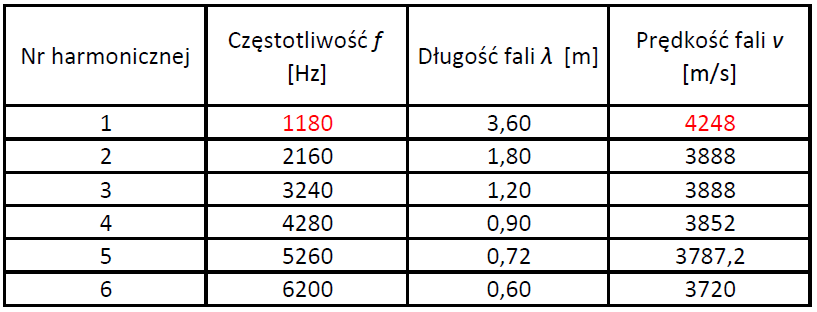
\includegraphics[width=0.7\textwidth]{tabmiedz}
		\label{fig:tabmiedz}
	\end{figure}
	\begin{figure}[!h]
		\centering
		\caption{Pomiary dla materiału aluminiowego.}
		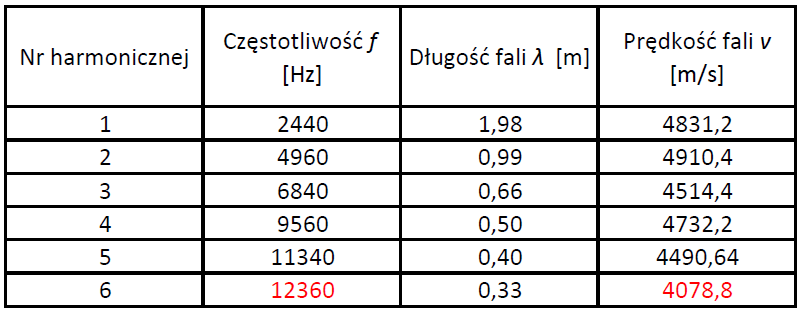
\includegraphics[width=0.7\textwidth]{tabaluminium}
		\label{fig:tabaluminium}
	\end{figure}
	\begin{figure}[!h]
		\centering
		\caption{Pomiary dla materiału mosiężnego.}
		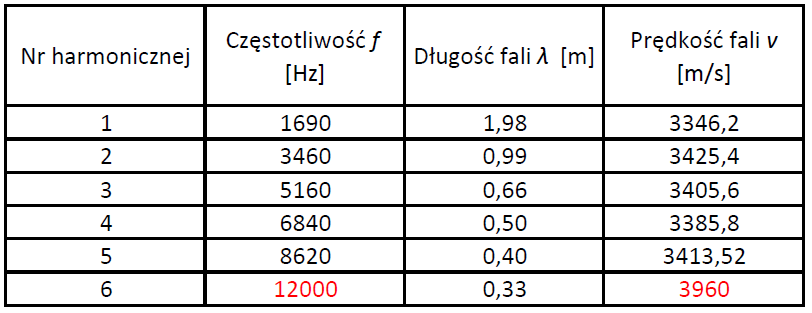
\includegraphics[width=0.7\textwidth]{tabmosiadz}
		\label{fig:tabmosiadz}
	\end{figure}
	\begin{figure}[!h]
		\centering
		\caption{Pomiary dla materiału stalowego.}
		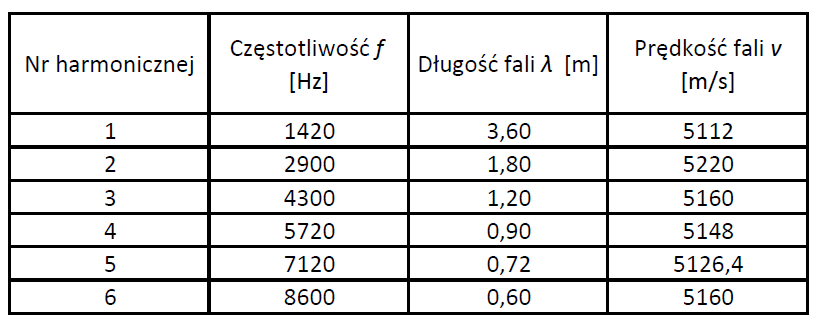
\includegraphics[width=0.7\textwidth]{tabstal}
		\label{fig:tabstal}
	\end{figure}
	\subsection{Analiza błedów}
	Na czerwono zostały oznaczone pomiary, których prędkość znacząco odbiega od średniej. Utożsamiamy je z błedami grubymi, które najprawdopodniej są wynikiem błędnego odczytu częstotliwości. 

	\subsection{Pomiary i ich niepewności.}
		
		Wszystkie wielkości mierzyliśmy niewielką ilość razy, dlatego dla każdej z nich przyjmujemy ocenę niepewności typu B, co w naszym przypadku będzie odpowiadać dokładności przyrządu pomiarowego.\newline
		W każdym przypadku $u(f) = 20 \text{ Hz}$.
		\begin{table}[h!]
			\centering
			\caption{Niepewności standardowe miedzi}
			\label{tab:nsmiedz}
			\begin{tabular}{l|l|l|l|l|l}
				 Symbol & \textit{$d$} [mm]  & \textit{$d_w$} [mm]   & \textit{$l$} [mm]     &  \textit{$m$} [g]  \\ \hline
				 Wartość(niepewność) & 15,2(5)      & 17,9(5) & 1801(1) & 761(1) \\
			\end{tabular}
		\end{table}
	
		\begin{table}[h!]
			\centering
			\caption{Niepewności standardowe aluminium}
			\label{tab:nsaluminium}
			\begin{tabular}{l|l|l|l|l}
				Symbol & \textit{$h$} [mm]  & \textit{$d$} [mm]   & \textit{$l$} [mm]     &  \textit{$m$} [g]   \\ \hline
				Wartość(niepewność) & 43,9(5)      & 4,9(5) & 999(1) & 23,89(1) \\
			\end{tabular}
		\end{table}
		
		\begin{table}[h!]
			\centering
			\caption{Niepewności standardowe stal}
			\label{tab:nsstal}
			\begin{tabular}{l|l|l|l|l}
				Symbol & \textit{$h$} [mm]  & \textit{$b$} [mm]   & \textit{$c$} [mm]  &  \textit{$m$} [g]   \\ \hline
				Wartość(niepewność) &19,8(5) & 14,1(5)      & 14,2(5) & 30,86(1) \\
			\end{tabular}
		\end{table}
	
		\begin{table}[h!]
			\centering
			\caption{Niepewności standardowe mosiadz}
			\label{tab:nsmosiadz}
			\begin{tabular}{l|l|l|l|l}
					Symbol & \textit{$d$} [mm]  & \textit{$h$} [mm]   & \textit{$l$} [mm]     & \textit{$m$} [g]   \\ \hline
				Wartość(niepewność)	& 5,9(5)      & 31,1(5) & 1800(1) & 74(1) \\
			\end{tabular}
		\end{table}
	Niepewność złożona powierzchni prostokąta:
		\begin{equation}
		u(P_P)=\sqrt{\bigg(\frac{\partial P_P}{\partial b}u(b)\bigg)^2 + \bigg(\frac{\partial P_p}{\partial a}u(a)\bigg)^2} = \sqrt{\bigg(bu(a)\bigg)^2+\bigg(au(b) \bigg)^2}
			\end{equation}
			
	Niepewność złożona powierzchni koła:
		\begin{equation}
		u(P_p)=\sqrt{\bigg(\frac{\partial P_P}{\partial d}u(d)\bigg)^2} = \sqrt{\bigg(\frac{\pi}{2}du(d)\bigg)^2}
		\end{equation}
		
	Niepewność złożona objętości:
	\begin{equation}
	u(V)=\sqrt{\bigg(\frac{\partial V}{\partial h}u(h)\bigg)^2 + \bigg(\frac{\partial V}{\partial P_p}u(P_p)\bigg)^2} = \sqrt{\bigg(hu(P_p)\bigg)^2+\bigg(P_pu(h) \bigg)^2}
	\end{equation}
	
	Niepewność złożona gęstości:
	\begin{equation}
	u(\rho)=\sqrt{\bigg(\frac{\partial \rho}{\partial V}u(V)\bigg)^2+\bigg(\frac{\partial \rho}{\partial \lambda}u(\lambda)\bigg)^2}=\sqrt{\bigg(-\frac{m}{V^2}u(V)\bigg)^2+\bigg(\frac{1}{V}u(m) \bigg)^2}
	\end{equation}
	
	Niepewność złożona prędkości:
	\begin{equation}
	u(v)=\sqrt{\bigg(\frac{\partial v}{\partial f}u(f)\bigg)^2+\bigg(\frac{\partial v}{\partial \lambda}u(\lambda)\bigg)^2}=\sqrt{\bigg(\lambda u(f)\bigg)^2+\bigg(f u(\lambda)\bigg)^2}
	\end{equation}
	
	Niepewność złożona modułu Younga:
	\begin{equation}
			 u(E)=\sqrt{\bigg(\frac{\partial E}{\partial \rho}u(\rho)\bigg)^2+\bigg(\frac{\partial E}{\partial v}u(v)\bigg)^2} =
	\sqrt{\bigg(v^2 u(\rho)\bigg)^2+\bigg(2 \rho v u(v)\bigg)^2}
	\end{equation}


	Korzystając z odpowiednich wzorów(zależnych od kszatłtu próbki) obliczamy niepewność złożoną modułu Younga dla wszystkich metali. 

		

	\section{Podsumowanie}
	\begin{center}
		\begin{tabular}{|c|c|c|c|c|c|}
			\hline Opis wielkości & $ E_0 \left[ \text{GPa} \right]$ & $E \left[ \text{GPa} \right]$ & $U(E) \left[ \text{GPa} \right]$ & $ \frac{u(E)}{E} $\\
			\hline Mosiądz  & 100 &  100,3& 4,93 & 2,46 \%  \\
			\hline Stal & 210-220 & 215,5 & 5,55 & 1,29 \%  \\  
			\hline Aluminium& 70 &  63,6&2,82  &  2,21 \%  \\ 
			\hline  Miedź& 110-130 & 86,4  &  4,86 & 2,81\% \\ 
			\hline 
		\end{tabular} 
	\end{center}
\vspace{1em}

\begin{itemize}
	\item Zarówno dla mosiądzu jak i dla stali otrzymane przez nas wyniki pokrywają się z wartościami tabelarycznymi. Świadczy to o poprawności wykonanych pomiarów.
	
	\item W przypadku aluminium uzyskany wynik, nawet po uwzględnieniu niepewności rozszerzonej, nie pokrywa się z wartością dokładną. Te pomiary zostały dokonane jako pierwsze i odczytwane wartości częstotliwości nie są dokładne. Mamy tutaj do czynienia z błedem systematycznym, wynikającym z nieodpowiednio umieszczoną skalą w oprogramowaniu. Po uwzględnieniu przesunięcia o +200 Hz (o taką różnicę podejrzewamy odczyt ze skali i odczyt myszą) moduł Younga równa się: $E=68,6 \pm 3 $ Gpa, co jest wynikiem poprawnym w zakresie obliczonej niepewności.
	
	\item Najgorsze wyniki otrzymaliśmy dla miedzi. Przyczną tak dużej rozbieżności jest najprawdopodobniej źle obliczona gęstość, której wartość dla naszych pomiarów wynosi $\rho=5900 \pm 304 \text{ }\mathrm{\frac{kg}{m^3}}$  , przy wartości tabelarycznej wynoszącej $\rho_0= 8900 \text{ }\mathrm{\frac{kg}{m^3}}$. Po zamianie gęstości na dokładną moduł Younga badanej próbki miedzi jest równy: $E=130 \pm 6 $GPa, co jest zgodne z wartością tabelaryczną w zakresie obliczonej niepewności. Możemy przypuszczać, że dokonaliśmy złych pomiarów rurki miedzianej, lub ewentualnie była ona wykonana z innego metalu.
\end{itemize}

\end{document}